\documentclass[a4paper, 8pt]{article}
\title{\textcolor{red}{Certificate Manager}}
\usepackage{listings}
\usepackage{color}
\usepackage{transparent}
\usepackage{enumitem}
\usepackage{graphicx,subfig}
\definecolor{dkgreen}{rgb}{0,0.6,0}
\definecolor{gray}{rgb}{0.5,0.5,0.5}
\definecolor{mauve}{rgb}{0.58,0,0.82}
\lstset{frame=tb,
  language=python,
  aboveskip=3mm,
  belowskip=3mm,
  showstringspaces=false,
  columns=flexible,
  basicstyle={\small\ttfamily},
  numbers=none,
  numberstyle=\tiny\color{gray},
  keywordstyle=\color{blue},
  commentstyle=\color{dkgreen},
  stringstyle=\color{mauve},
  breaklines=true,
  breakatwhitespace=true,
  tabsize=3
}
\begin{document}
\maketitle
\tableofcontents
\section{Introduction}
Certificate Manager is the first subsystem that needs to be configured in PKI Environment, Certificate Manager can be configured as RootCA, Subordinate CA
\begin{enumerate}[label*=\arabic*.]
    \item Key features:
    \begin{itemize}
        \item CA subsystem issues, renews, revokes Certificates, generates Certificat Revocation lists
        \item Publishes Certificates/CRL in form of files or can publish to LDAP or OCSP responder
        \item CA also has an inbuilt OCSP responder enabling OCSP-Compliant clients to query CA about revocation status of Certificate
        \item Some CA's can delegate some of it's responsibility to another Subordinate CA
    \end{itemize}
\item Generic Architecture
    \begin{figure}[ht!]
        \centering
        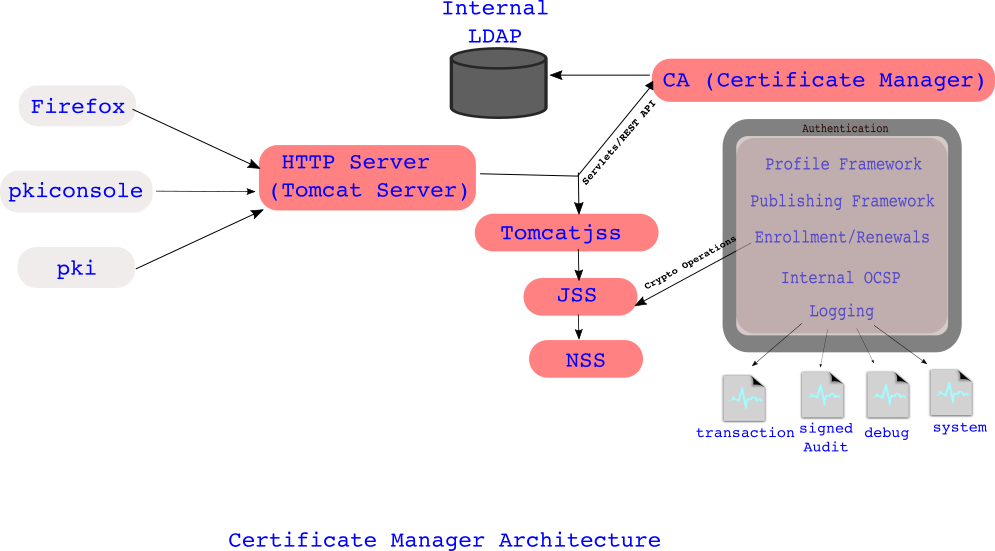
\includegraphics[width=120mm]{Images/CA-subsystem-Arch3.png}
        \caption{CA Subsystem Architecture}
    \end{figure}
\item Interfaces
    \begin{itemize}
        \item End User Interface(Browser/CLI)
        \item Agent Interface(Browser/CLI)
        \item Admin interface(java console)
    \end{itemize}
\item Features
\end{enumerate}
\end{document}

